%!TEX root = ../../thesis.tex

The non-\WW diboson background comprises the \Wgamma, \Wgstar, \WZ and \ZZ processes (ordered 
by contribution to the signal region). \Wgamma events feature a prompt photon that passes the 
electron selection, via an asymmetric conversion (\epluseminus production). The other 
processes have signatures of \HepProcess{\Plepton\Pnu\Plepton\Plepton}, 
\HepProcess{\Plepton\Plepton\Plepton\Plepton} or \HepProcess{\Plepton\Plepton\Pnu\Pnu}, and 
usually contribute when additional leptons fail object selection 
(\eg \unit{$\pt < 10$}{\GeV}).



\subsection{Same-sign control region}
\label{sec:diboson:sscr}

In non-\WW diboson backgrounds, a symmetry is expected to exist between opposite-sign (OS) 
and same-sign (SS) dilepton events; asymmetric processes such as \HepProcess{\PZ\PZ \HepTo 
\Plepton\Plepton\Pnu\Pnu} have negligible contribution. Conversely, the \WW, top and \DY 
backgrounds only contribute to the OS sample. Finally, the \Wjets background displays a 
partial OS/SS symmetry (see \ref{sec:wjets:wjet_bkg}). Thus, SS events can be used to 
estimate the non-\WW diboson background in the OS signal region, whilst validating the \Wjets 
estimation.

An SS control region (CR) is defined using identical criteria to the OS signal region (SR). 
In the language of \Section~\ref{sec:wjets}, the SS CR events are in the SR of the SS 
dilepton sample $\mathcal{N}_{\id{\Plepton}\id{\Plepton}\text{,SS}}$. This is used to 
determine the normalisation of the non-\WW diboson background, whilst the shapes of 
distributions used in the fitting procedure (\ie \mt, \mll and \ptsubleadlep) are modelled by 
MC. This is equivalent to
\begin{equation}
	N_{\HepProcess{\PV\PV}}^{\text{pred,SR}} &= \alpha_{\HepProcess{\PV\PV}} \cdot \parenths{N^{\text{data,CR}} - N_{\text{non-}\HepProcess{\PV\PV}}^{\text{pred,CR}}} \label{eq:sscr} \\
	\alpha_{\HepProcess{\PV\PV}} &= N_{\HepProcess{\PV\PV}}^{\text{MC,SR}} / N_{\HepProcess{\PV\PV}}^{\text{MC,CR}}
\end{equation}
where $\HepProcess{\PV\PV} = \Wgamma + \Wgstar + \WZ + \ZZ$ and 
$N_{\text{non-}\HepProcess{\PV\PV}}^{\text{pred,CR}}$ is dominated by \Wjets. This SS CR 
method is used in the \emch/\mech channels of the 0-jet and 1-jet bins, whilst the other 
signal regions model the non-\WW diboson background with MC.

Uncertainties in the sizes of the constituent processes will cancel if the composition of the 
non-\WW diboson background is the same in SS and OS events; this is modelled by MC. However, 
uncertainties in the shapes of distributions remain, since these are not constrained by the 
SS CR method. Additionally, the uncertainty component of the OS \Wjets background that is 
correlated between OS and SS will cancel in the SS CR method; an increase in the SS \Wjets 
background will be compensated by a decrease in the non-\WW diboson background, and vice 
versa.

To estimate the non-\WW diboson background in regions other than the SR, the method is viewed 
as providing a simple data-driven normalisation factor. This is equivalent to neglecting the 
extrapolation uncertainties, but is helpful when plotting observables. The normalisation 
factors are measured to be \stat{0.96}{0.07} in the 0-jet bin and \stat{0.93}{0.13} in the 
1-jet bin\todo{update}. 

\Figure~\ref{fig:sscr} validates the MC shape modelling of the fit observables in the SS CRs, 
following application of the normalisation factors. Good agreement with experimental data is 
observed. Note that these SS distributions are not directly used, since only the total number 
of events in the SS CRs are used in (\ref{eq:sscr}).

\begin{figure}[p]
	\includegraphics[width=0.48\textwidth]{tex/backgrounds/emme_CutFRecoil_0jet_sscr_MT_TrackHWW_Clj_mh125_lin}
	\hfill
	\includegraphics[width=0.48\textwidth]{tex/backgrounds/emme_CutFRecoil_1jet_sscr_MT_TrackHWW_Clj_mh125_lin}
	\\
	\includegraphics[width=0.48\textwidth]{tex/backgrounds/emme_CutFRecoil_0jet_sscr_Mll_zoom_mh125_lin}
	\hfill
	\includegraphics[width=0.48\textwidth]{tex/backgrounds/emme_CutFRecoil_1jet_sscr_Mll_zoom_mh125_lin}
	\\
	\includegraphics[width=0.48\textwidth]{tex/backgrounds/emme_CutFRecoil_0jet_sscr_lepPtSubLead_zoom_mh125_lin}
	\hfill
	\includegraphics[width=0.48\textwidth]{tex/backgrounds/emme_CutFRecoil_1jet_sscr_lepPtSubLead_zoom_mh125_lin}
	\caption{The \mt (top), \mll (middle) and \ptsubleadlep (bottom) distributions in the 
	0-jet (left) and 1-jet (right) same-sign control regions. Normalisation factors are 
	applied.}
	\label{fig:sscr}
\end{figure}



\subsection{\Wgamma}
\label{sec:diboson:wgamma}

\Wgamma events enter the dilepton sample when the photon fakes an electron. This is usually 
caused by an asymmetric \HepProcess{\Pphoton \HepTo \epluseminus} conversion, where only one 
electron passes the object selection. This background is suppressed via the electron 
identification criteria, which require a hit in the first pixel layer and no conversion 
vertex (see \Section~\ref{sec:objects:electrons}).

\Wgamma is modelled by \meps{\alpgen}{\fherwig} and normalised to the NLO cross section 
calculated with \mcfm. Modelling is tested with a SS dilepton sample of \emch/\mech events, 
but where the electron object is required to have a conversion vertex and no hit in the first 
pixel layer (\ie the photon rejection criteria are inverted). Validation regions (VRs) are 
defined in the 0-jet and 1-jet bins, using the corresponding signal region cuts. Experimental 
data is found to be well described, as seen in \Figure~\ref{fig:wgamma:vr}.

\begin{figure}[t]
	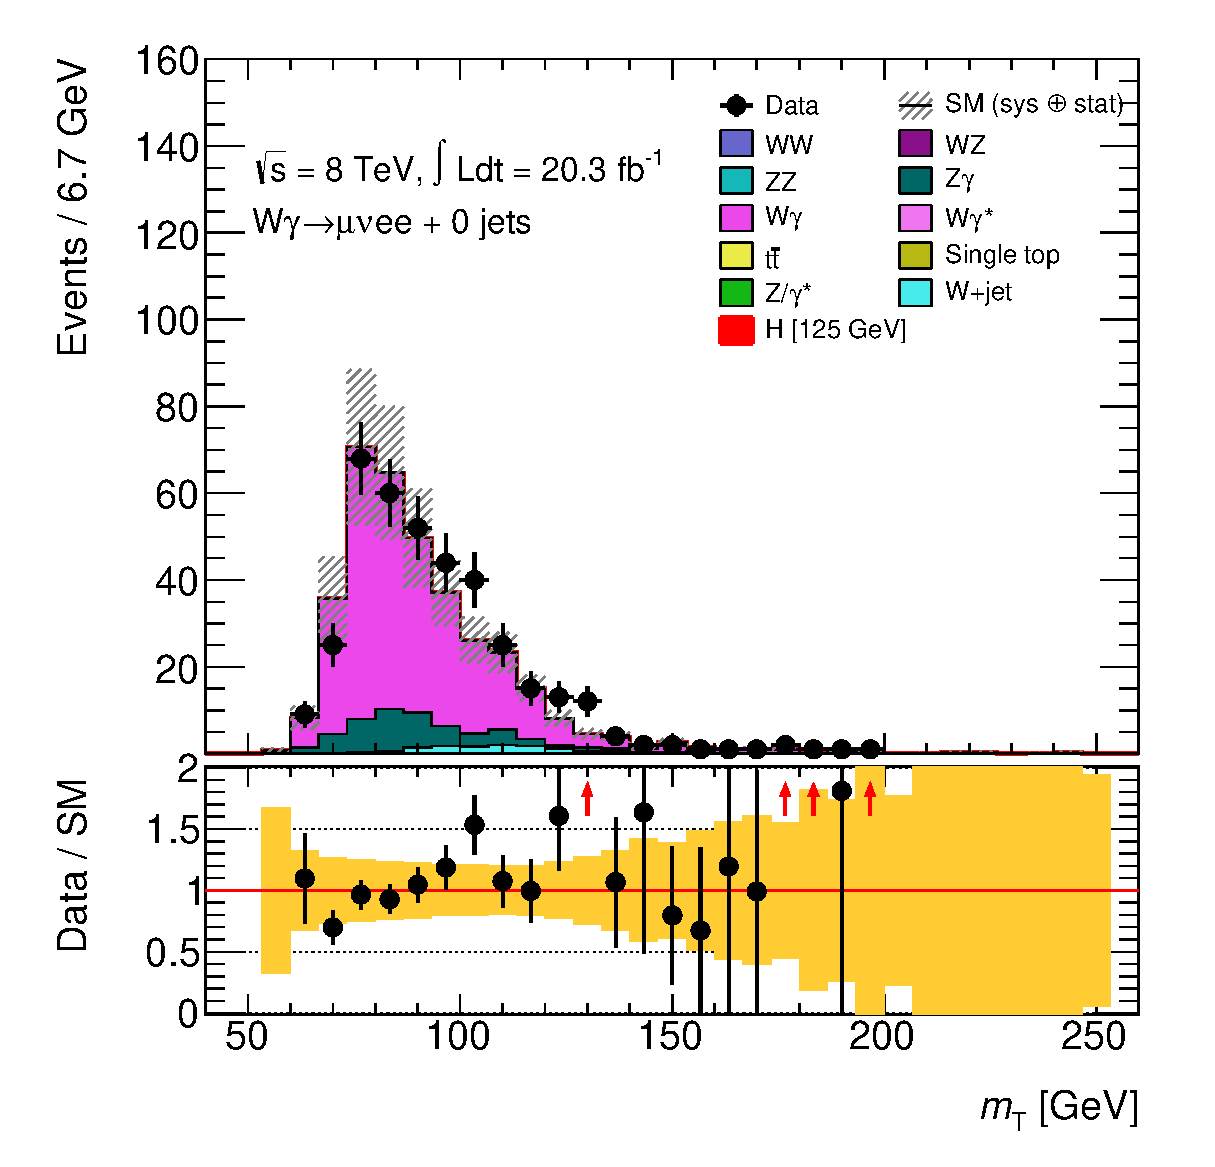
\includegraphics[width=0.48\textwidth]{tex/backgrounds/Wgamma/CutTopoDPhill_0jet_MT_TrackHWW_Clj_mh125_lin}
	\hfill
	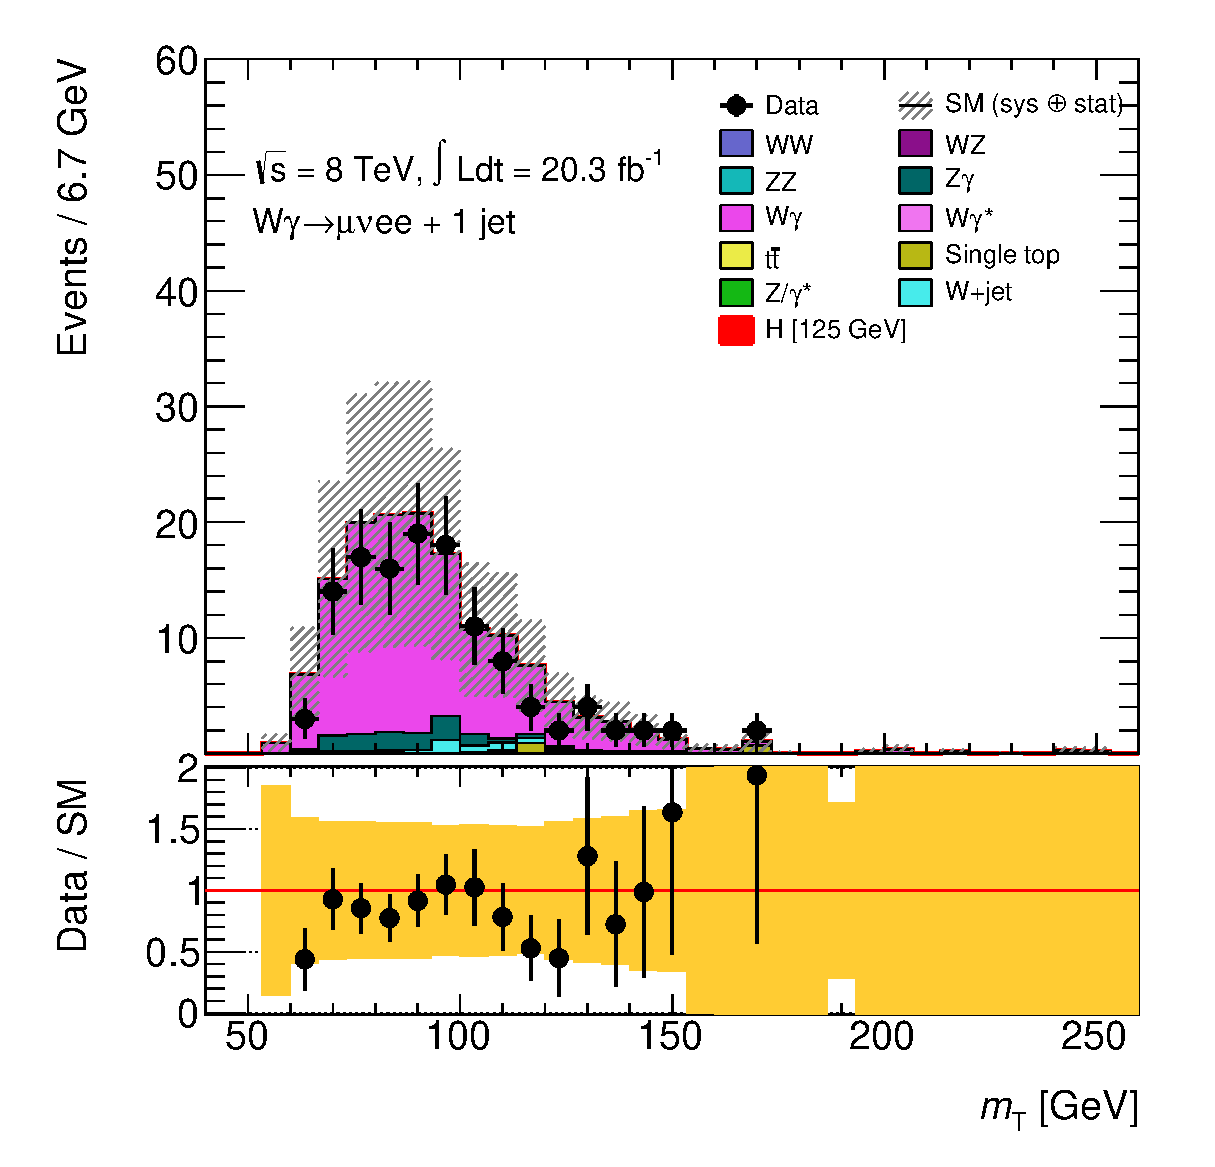
\includegraphics[width=0.48\textwidth]{tex/backgrounds/Wgamma/CutTopoDPhill_1jet_MT_TrackHWW_Clj_mh125_lin}
	\caption{The \mt distribution in the 0-jet (left) and 1-jet (right) \Wgamma validation 
	regions. The shaded error band includes statistical and theoretical uncertainties, in 
	addition to those associated with conversion modelling.}
	\label{fig:wgamma:vr}
\end{figure}

As the conversion and pixel hit criteria are inverted in the VR, their modelling is not 
tested in \Figure~\ref{fig:wgamma:vr}. Unfortunately, it is not possible to define a 
high-purity \Wgamma VR when including these criteria. Instead, 
a \HepProcess{\Zgamma \HepTo \Pmu\Pmu\Pphoton} VR is used to test this modelling. 
Events are selected with an OS muon pair with \unit{$p_{\text{T,\Pmu}}^{\text{lead}} > 
22$}{\GeV} and \unit{$p_{\text{T,\Pmu}}^{\text{sublead}} > 10$}{\GeV}, and an additional 
electron with \unit{$p_{\text{T,\Pe}} > 10$}{\GeV}. Low mass resonances are vetoed by 
\unit{$m_{\HepProcess{\Pmu\Pmu}} > 12$}{\GeV}, and events featuring QED FSR are selected by 
\unit{$\mods{m_{\HepProcess{\Pmu\Pmu\Pe}} - \mZ} < 15$}{\GeV}. The selected events are 
\about60\% \Zgamma and \about40\% \Zgstar. The mismodelling is found to depend upon 
$p_{\text{T,\Pe}}$ and so a conversion systematic uncertainty is derived: 25\% for 
\unit{10 -- 15}{\GeV}, 18\% for \unit{15 -- 20}{\GeV} and 5\% for \unit{$>\!20$}{\GeV}.



\subsection{\WZ and \Wgstar}
\label{sec:diboson:wgstar}

% separated into 2 samples
% WZ K-factor from MCFM
% Wgstar difficult to simulate low mass, must extrapolate K-factor
% usual stuff from theory note
% Wgstar VR

\begin{figure}[p]
	\includegraphics[width=0.495\textwidth]{tex/backgrounds/Wgstar/em_CutDPhiMax_lepPtSublead_zoom_mh125_lin}
	\hfill
	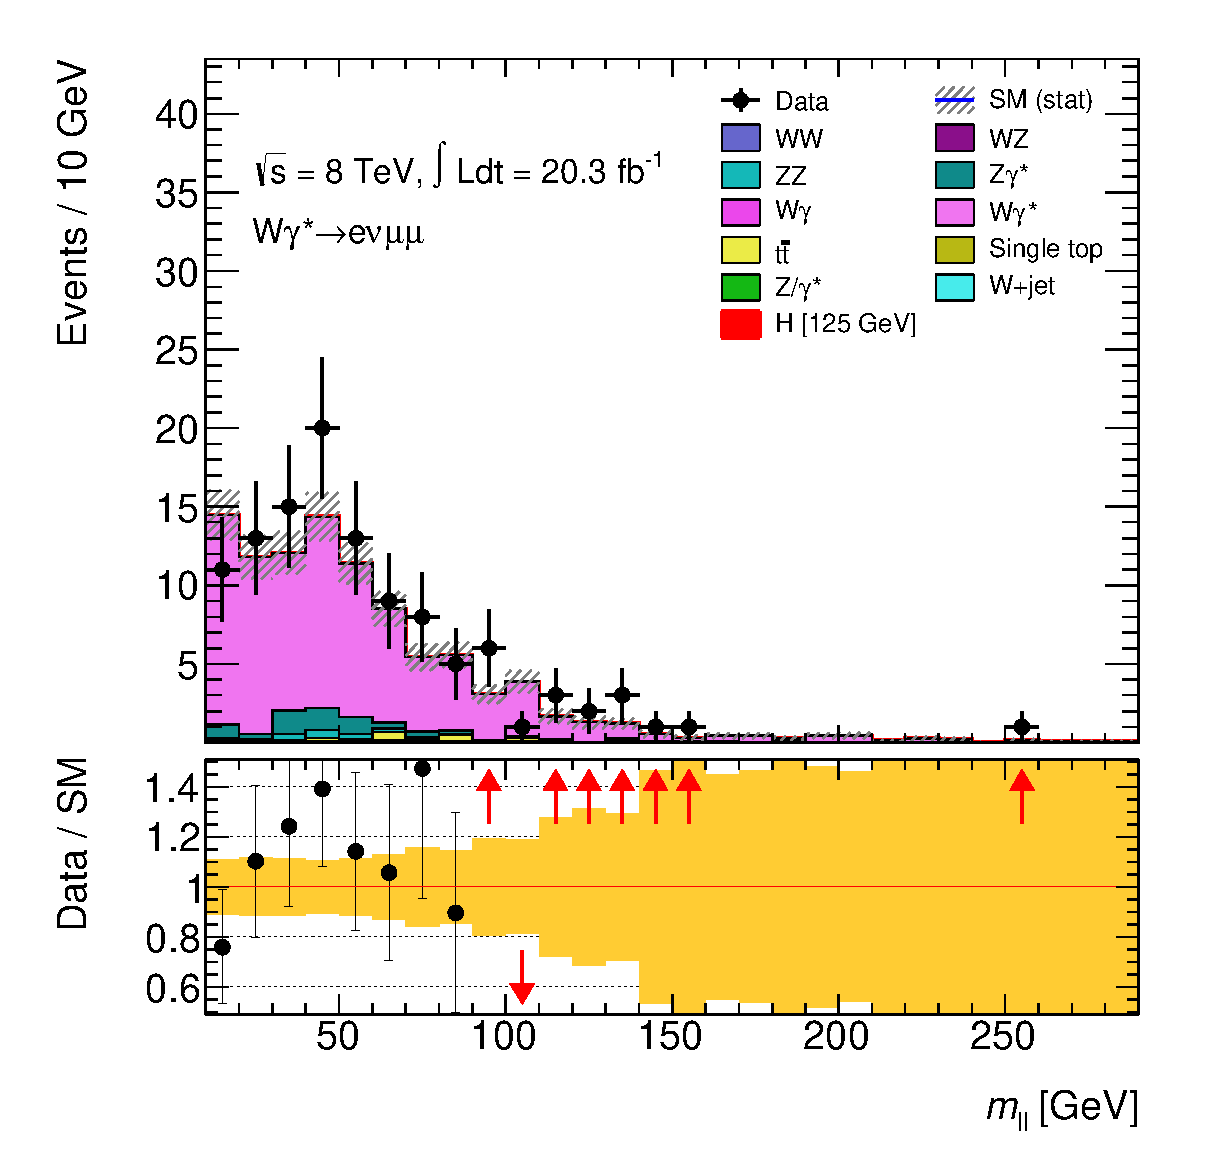
\includegraphics[width=0.495\textwidth]{tex/backgrounds/Wgstar/em_CutDPhiMax_Mll_mh125_lin}
	\\
	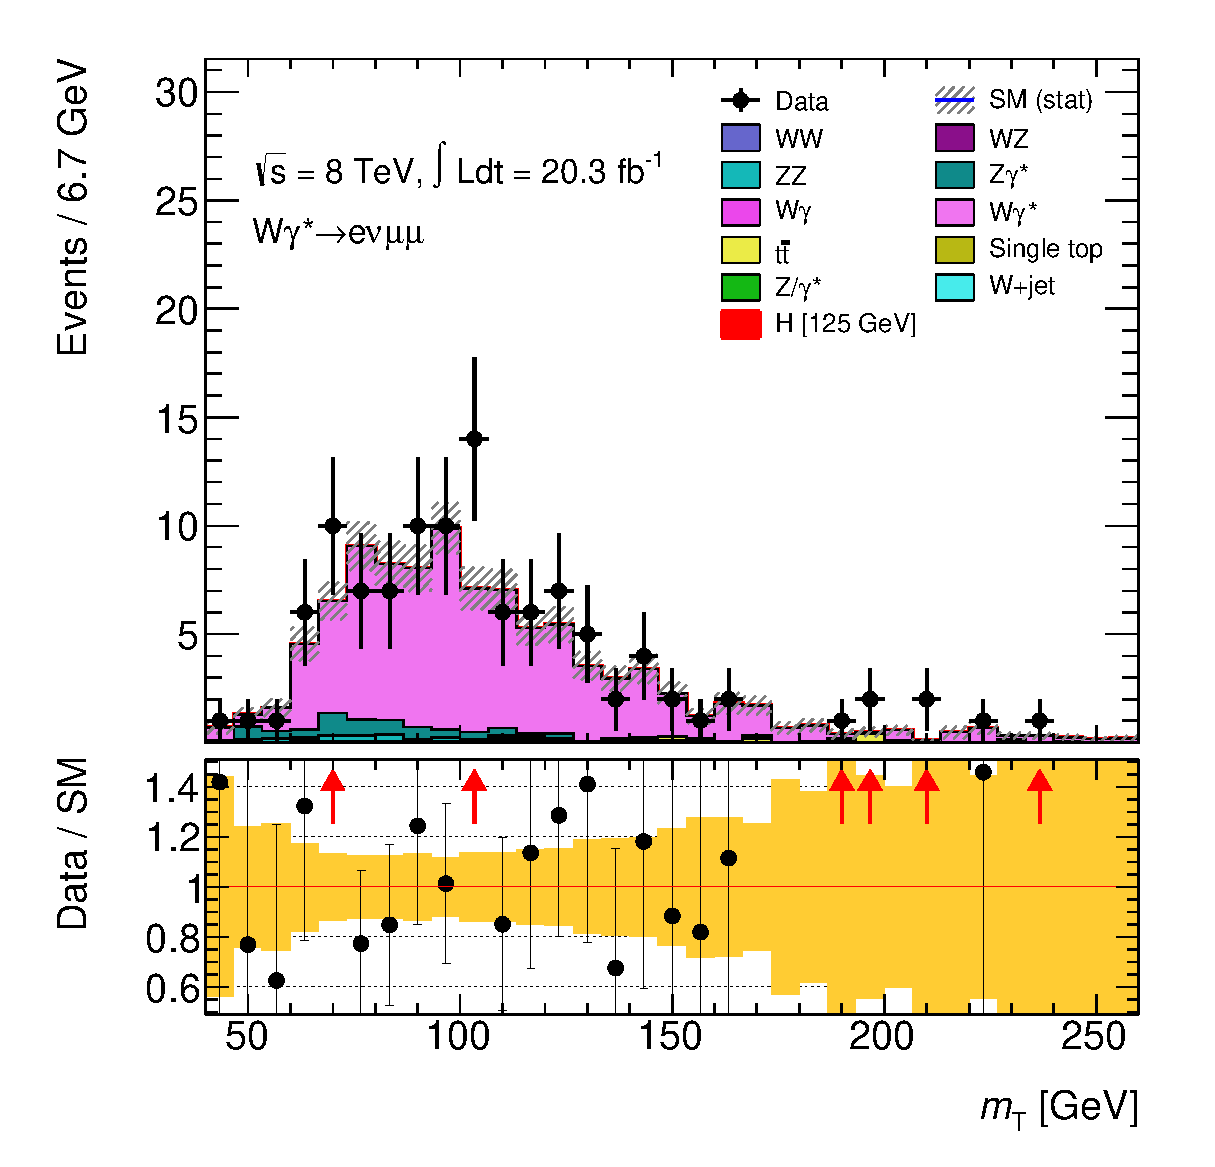
\includegraphics[width=0.495\textwidth]{tex/backgrounds/Wgstar/em_CutDPhiMax_MT_TrackHWW_Clj_mh125_lin}
	\hfill
	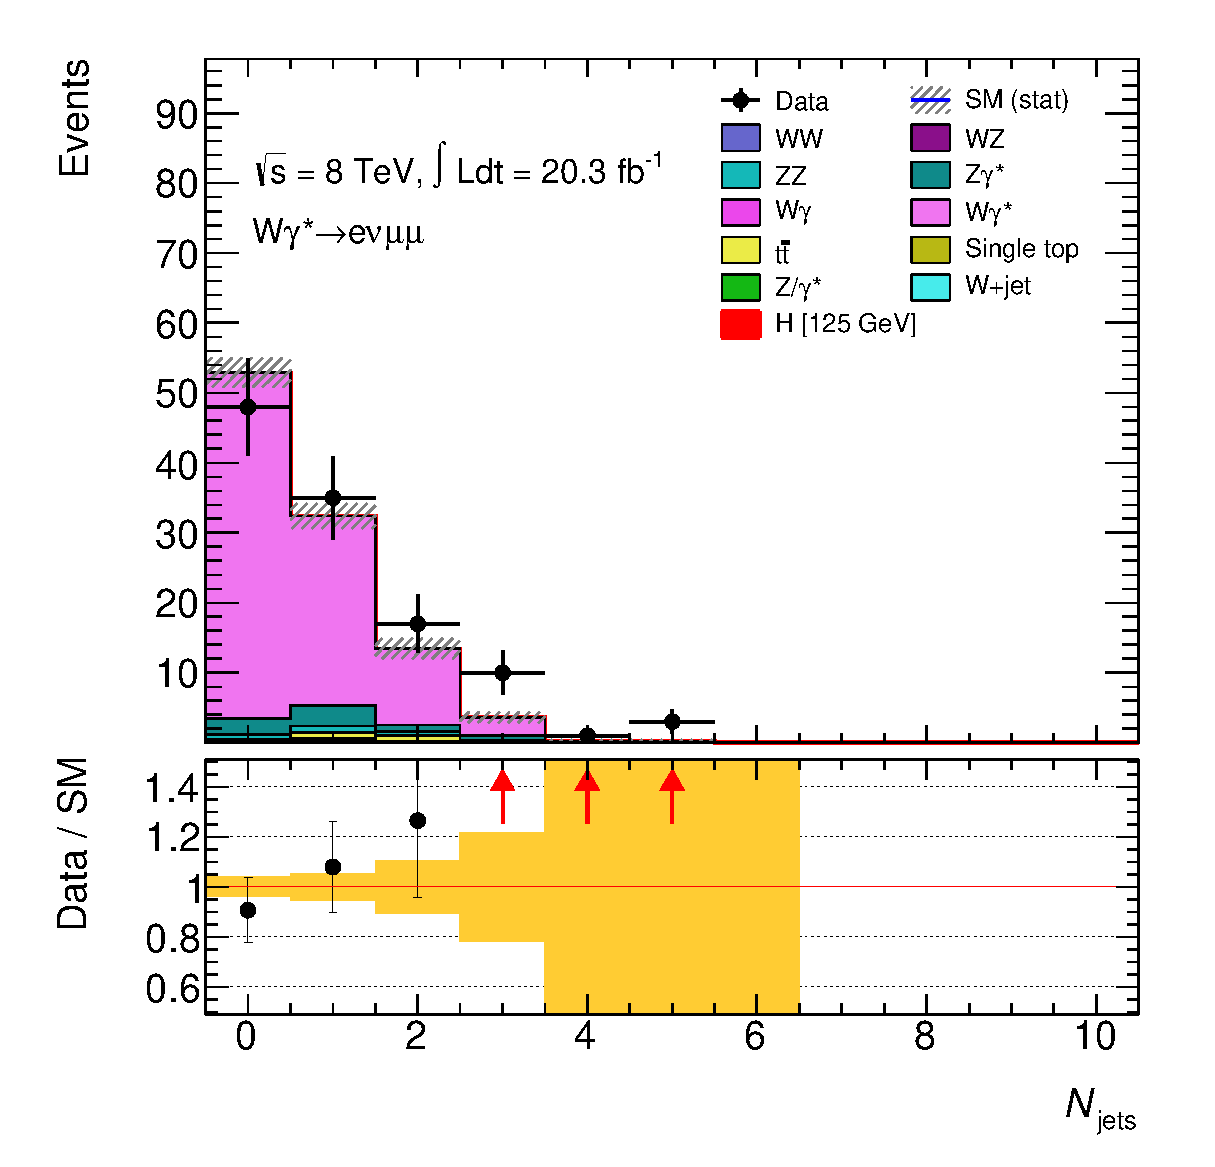
\includegraphics[width=0.495\textwidth]{tex/backgrounds/Wgstar/em_CutDPhiMax_m_jet_n_mh125_lin}
	\caption{}
	\label{fig:wgstar:vr}
\end{figure}


\subsection{\ZZ and \Zgstar}
\label{sec:diboson:zz}

% Zg* used in electroweak subtraction when calculating Z+jet fake factor
